% !TEX TS-program = lualatex
% !BIB TS-program = biber
%\documentclass[handout]{beamer}
\documentclass{beamer}
\input{../common/misomva}
\newcommand{\misoclasstinytitleslide}{Partially based on material by:  Mikhail Belkin, \\[-1em] 
Jerry Zhu, Olivier Chapelle, Branislav Kveton}
\newcommand{\misoclassdate}{}
\begin{document}
% Topic-specific title slide
\newcommand{\topictitle}{Inductive Generalization Bounds}
\newcommand{\topicsubtitle}{Theoretical Guarantees for Inductive SSL}
\renewcommand{\misoclasstinytitleslide}{Partially based on material by:  Mikhail Belkin, Partha Niyogi, \\[-1em] Olivier Chapelle, Bernhard Sch\"olkopf}

\MakeTopicSlide

\begin{frame}
\frametitle{Inductive Generalization Bounds}
%\pause
We may want to bound the \emphcol{risk}
\begin{equation*}%[Risk of our solutions]
  R_P(f) = \EEs{P(\bx)}{\cL\left(f\left(\bx\right), y\left(\bx\right)\right)}
\end{equation*}
\pause
for some \emphcol{loss}, e.g.,~0/1 loss
\[
\cL(y', y) \! = \! \1\{\sgn(y') \! \neq \! y\}
\]
\pause 
\vspace{-1em}
%\pause 
\begin{center}
$R_P(f) \leq \hat{R}_P(f) + \emphcol{error terms}$
\end{center}
\end{frame}
%%%%%%%%%%%%%%%%%%%%%%%%%%%%%%%%%%%%%%%%%%%%%%%%%%%%%%%%%%%%

\begin{frame}
\frametitle{Inductive Generalization Bounds}

Using classical SLT tools (Equations 3.15 and 3.24~\cite{vapnik1995nature}),
with probability  $1 - \mcolA{\eta}$
\begin{align*}
  R_P(f) \leq \frac{1}{\mcolB{N}} \sum_i \cL(f(\bx_i), y_i) +
  \Delta_I(\alert{h}, \mcolB{N}, \mcolA{\eta}).
\end{align*}

\pause
$\mcolB{N} \equiv $ number of samples
\pause
, $\alert{h} \equiv $ VC dimension of the class 
\pause
\[
\Delta_I(\alert{h}, \mcolB{N}, \mcolA{\eta}) =\sqrt{\frac{ \alert{h}  (\ln(2 \mcolB{N} / \alert{h}) + 1) - \ln(\mcolA{\eta} / 4)}{\mcolB{N}}}
\]

\pause
\bskip
\questionbox{ How to bound $\cL(f(\bx_i), y_i)$?}
\end{frame}

\begin{frame}
\frametitle{Inductive Generalization Bounds}

For any $y_i \in \set{-1, 1}$ and $\ell_i^\star$
\begin{align*}
&\frac{1}{\mcolB{N}} \sum_i \cL(f(\bx_i), y_i)
\leq \frac{1}{\mcolB{N}} \sum_i\cL(f(\bx_i), \sgn(\ell_i^\star))
+ \frac{1}{\mcolB{N}} \sum_i{(\ell_i^\star - y_i)^2}\\
\onslide<2->{&\leq \left(\frac{1}{\mcolB{N}} \sum_i \cL(f(\bx_i), \sgn(\ell_i^\star))\right) + {\widehat{R}_P(\bell^\star) +
  \Delta_T(\beta, n_l, \delta)}}
\end{align*}
\end{frame}
%%%%%%%%%%%%%%%%%%%%%%%%%%%%%%%%%%%%%%%%%%%%%%%%%%%%%%%%%%%%
%%%%%%%%%%%%%%%%%%%%%%%%%%%%%%%%%%%%%%%%%%%%%%%%%%%%%%%%%%%%
\begin{frame}
\frametitle{Inductive Generalization Bounds}
\textbf{Combining  \emphcol{inductive} +  \emphcol{transductive} error} 
\moveb
With probability $1 - (\eta + \delta)$.
\begin{align*}
  R_P(f)
  \ \leq & \ \
  \frac{1}{N} \sum_i \cL(f(\bx_i), \sgn(\ell_i^\star)) \ + \\
  & \ \
  \widehat{R}_P(\bell^\star) +
  \Delta_T(\beta, n_l, \delta) + \Delta_I(h, N, \eta)
\end{align*}

\pause We need to account for $\eps$. With probability $1 - (\eta + \delta)$.
\begin{align*}
  R_P(f) \leq & 
  \frac{1}{N} \!\!\! \sum_{i : \abs{\ell_i^\star} \geq \eps}
  \!\!\! \cL(f(\bx_i), \sgn(\ell_i^\star)) +
  \frac{2 \eps n_\eps}{N} + \\
  & \ \
  \widehat{R}_P(\bell^\star) +
  \Delta_T(\beta, n_l, \delta) + \Delta_I(h, N, \eta)
\end{align*}
\pause 
\vspace{-1em}
\rightyellbox{We should have $\varepsilon \leq n_l^{-1/2}$!}

\end{frame}


%%%%%%%%%%%%%%%%%%%%%%%%%%%%%%%%%%%%%%%%%%%%%%%%%%%%%%%%%%%%
\begin{frame}
\frametitle{SSL with Graphs: LapSVMs and MM Graph Cuts}

\begin{center}
MMGC for 2D data and \textbf{linear} $\cK$ works as we want \bigskip \\ 
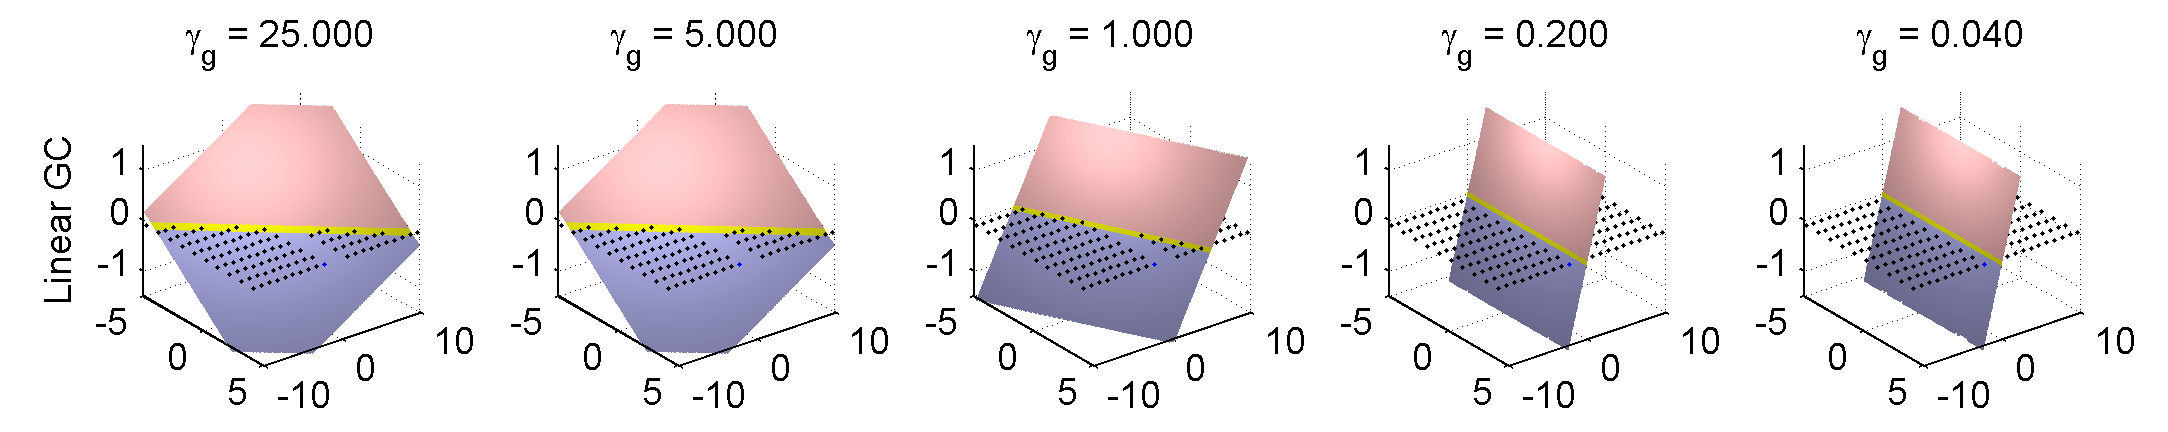
\includegraphics[width=\columnwidth]{../img/SyntheticCuts1a}\\
LSVM for 2D data and \textbf{linear} $\cK$ only changes the slope \\ \bigskip
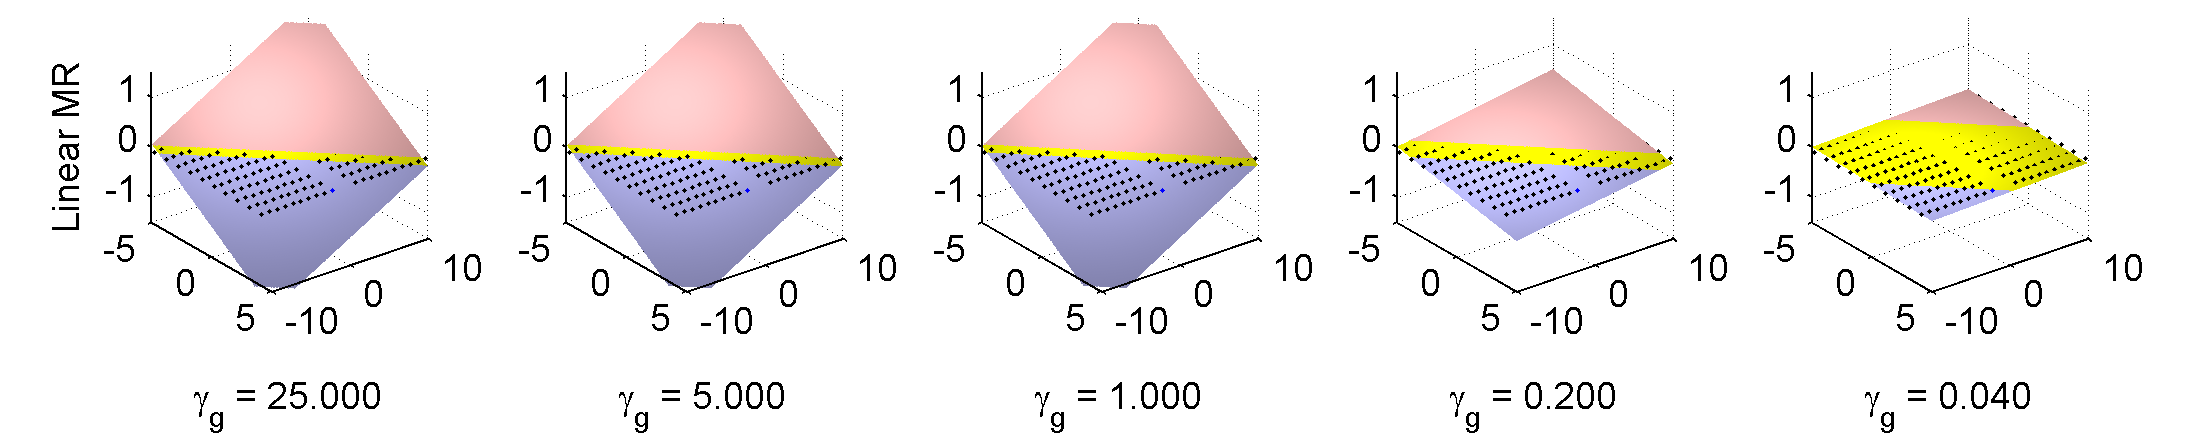
\includegraphics[width=\columnwidth]{../img/SyntheticCuts1b}
\end{center}

\end{frame}
%%%%%%%%%%%%%%%%%%%%%%%%%%%%%%%%%%%%%%%%%%%%%%%%%%%%%%%%%%%%
%%%%%%%%%%%%%%%%%%%%%%%%%%%%%%%%%%%%%%%%%%%%%%%%%%%%%%%%%%%%
\begin{frame}
\frametitle{SSL with Graphs: LapSVMs and MM Graph Cuts}

\begin{center}
LSVM for 2D data and \textbf{cubic} $\cK$ is also not so good\\ \bigskip
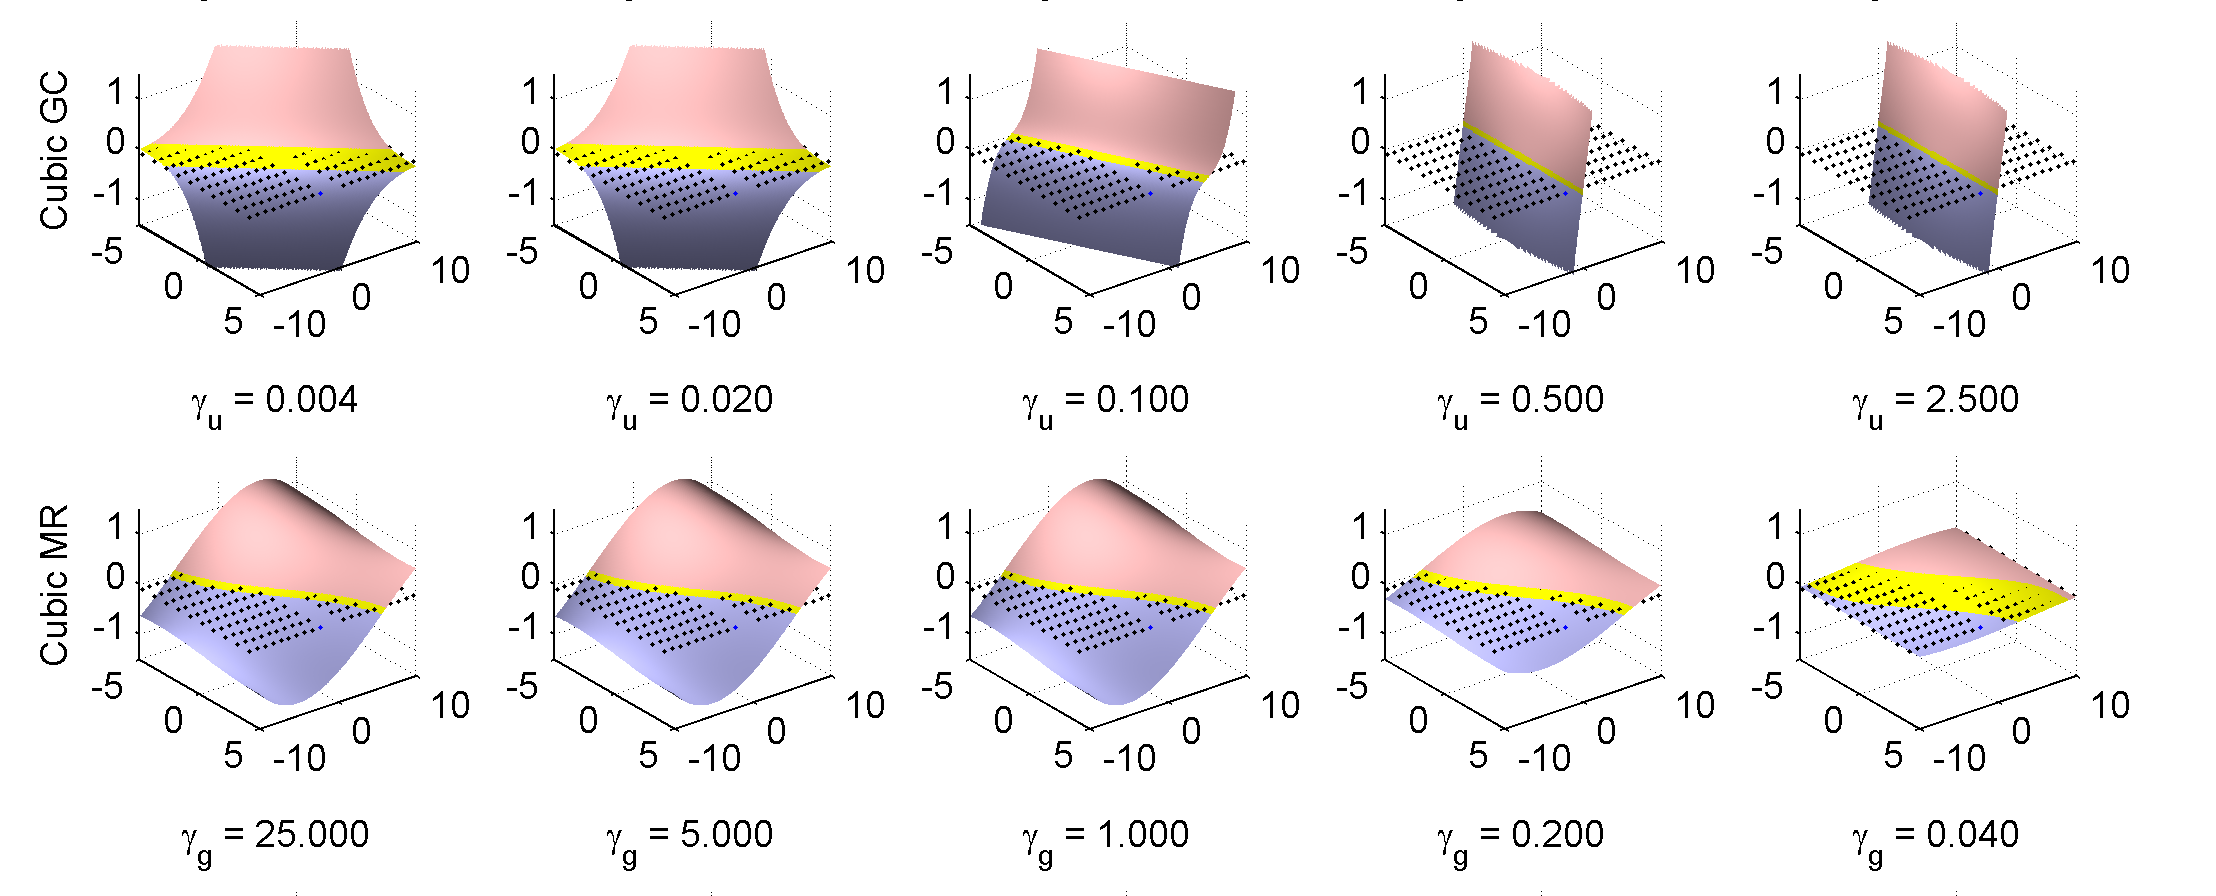
\includegraphics[width=\columnwidth]{../img/SyntheticCuts2}
\end{center}

\end{frame}
%%%%%%%%%%%%%%%%%%%%%%%%%%%%%%%%%%%%%%%%%%%%%%%%%%%%%%%%%%%%
%%%%%%%%%%%%%%%%%%%%%%%%%%%%%%%%%%%%%%%%%%%%%%%%%%%%%%%%%%%%
\begin{frame}
\frametitle{SSL with Graphs: LapSVMs and MM Graph Cuts}

\begin{center}
MMGC and LSVM for 2D data and RBF $\cK$  \\ \bigskip
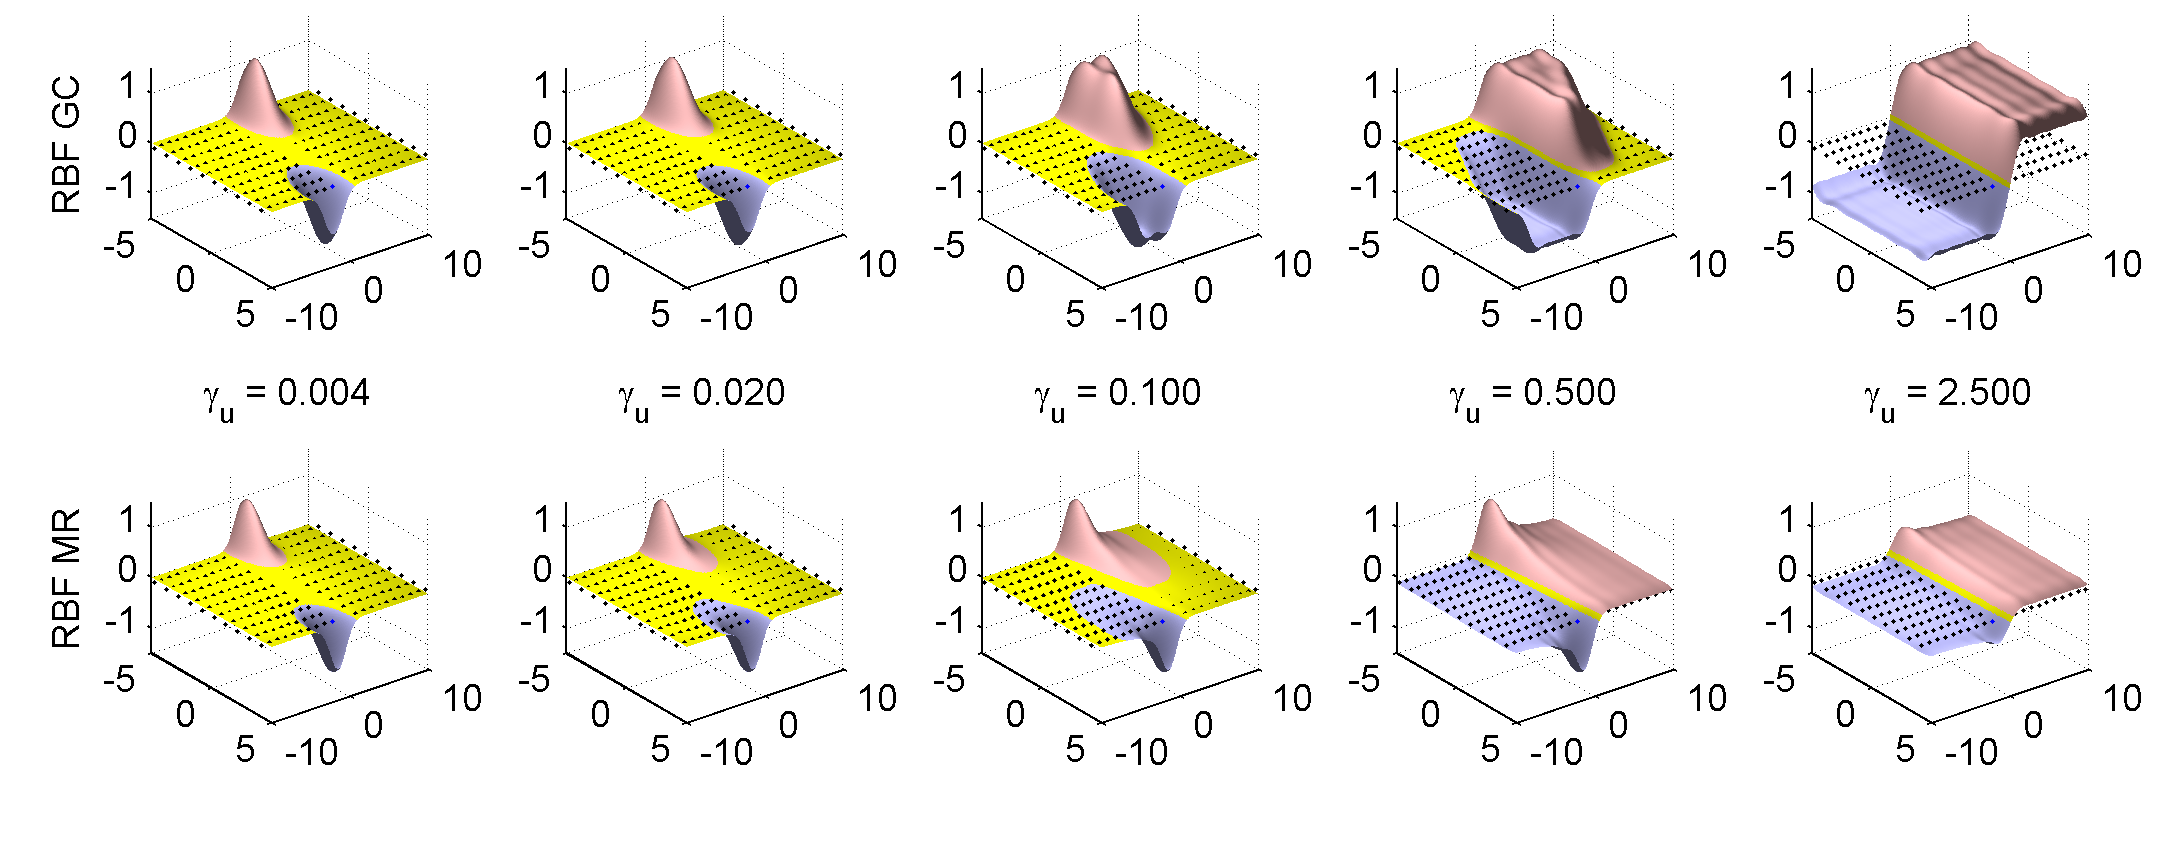
\includegraphics[width=\columnwidth]{../img/SyntheticCuts3}
\end{center}

\end{frame}
%%%%%%%%%%%%%%%%%%%%%%%%%%%%%%%%%%%%%%%%%%%%%%%%%%%%%%%%%%%%

%%%%%%%%%%%%%%%%%%%%%%%%%%%%%%%%%%%%%%%%%%%%%%%%%%%%%%%



\MakeLastSlide
\end{document}
